\documentclass[twoside]{book}

% Packages required by doxygen
\usepackage{fixltx2e}
\usepackage{calc}
\usepackage{doxygen}
\usepackage[export]{adjustbox} % also loads graphicx
\usepackage{graphicx}
\usepackage[utf8]{inputenc}
\usepackage{makeidx}
\usepackage{multicol}
\usepackage{multirow}
\PassOptionsToPackage{warn}{textcomp}
\usepackage{textcomp}
\usepackage[nointegrals]{wasysym}
\usepackage[table]{xcolor}

% Font selection
\usepackage[T1]{fontenc}
\usepackage[scaled=.90]{helvet}
\usepackage{courier}
\usepackage{amssymb}
\usepackage{sectsty}
\renewcommand{\familydefault}{\sfdefault}
\allsectionsfont{%
  \fontseries{bc}\selectfont%
  \color{darkgray}%
}
\renewcommand{\DoxyLabelFont}{%
  \fontseries{bc}\selectfont%
  \color{darkgray}%
}
\newcommand{\+}{\discretionary{\mbox{\scriptsize$\hookleftarrow$}}{}{}}

% Page & text layout
\usepackage{geometry}
\geometry{%
  a4paper,%
  top=2.5cm,%
  bottom=2.5cm,%
  left=2.5cm,%
  right=2.5cm%
}
\tolerance=750
\hfuzz=15pt
\hbadness=750
\setlength{\emergencystretch}{15pt}
\setlength{\parindent}{0cm}
\setlength{\parskip}{3ex plus 2ex minus 2ex}
\makeatletter
\renewcommand{\paragraph}{%
  \@startsection{paragraph}{4}{0ex}{-1.0ex}{1.0ex}{%
    \normalfont\normalsize\bfseries\SS@parafont%
  }%
}
\renewcommand{\subparagraph}{%
  \@startsection{subparagraph}{5}{0ex}{-1.0ex}{1.0ex}{%
    \normalfont\normalsize\bfseries\SS@subparafont%
  }%
}
\makeatother

% Headers & footers
\usepackage{fancyhdr}
\pagestyle{fancyplain}
\fancyhead[LE]{\fancyplain{}{\bfseries\thepage}}
\fancyhead[CE]{\fancyplain{}{}}
\fancyhead[RE]{\fancyplain{}{\bfseries\leftmark}}
\fancyhead[LO]{\fancyplain{}{\bfseries\rightmark}}
\fancyhead[CO]{\fancyplain{}{}}
\fancyhead[RO]{\fancyplain{}{\bfseries\thepage}}
\fancyfoot[LE]{\fancyplain{}{}}
\fancyfoot[CE]{\fancyplain{}{}}
\fancyfoot[RE]{\fancyplain{}{\bfseries\scriptsize Generated by Doxygen }}
\fancyfoot[LO]{\fancyplain{}{\bfseries\scriptsize Generated by Doxygen }}
\fancyfoot[CO]{\fancyplain{}{}}
\fancyfoot[RO]{\fancyplain{}{}}
\renewcommand{\footrulewidth}{0.4pt}
\renewcommand{\chaptermark}[1]{%
  \markboth{#1}{}%
}
\renewcommand{\sectionmark}[1]{%
  \markright{\thesection\ #1}%
}

% Indices & bibliography
\usepackage{natbib}
\usepackage[titles]{tocloft}
\setcounter{tocdepth}{3}
\setcounter{secnumdepth}{5}
\makeindex

% Hyperlinks (required, but should be loaded last)
\usepackage{ifpdf}
\ifpdf
  \usepackage[pdftex,pagebackref=true]{hyperref}
\else
  \usepackage[ps2pdf,pagebackref=true]{hyperref}
\fi
\hypersetup{%
  colorlinks=true,%
  linkcolor=blue,%
  citecolor=blue,%
  unicode%
}

% Custom commands
\newcommand{\clearemptydoublepage}{%
  \newpage{\pagestyle{empty}\cleardoublepage}%
}

\usepackage{caption}
\captionsetup{labelsep=space,justification=centering,font={bf},singlelinecheck=off,skip=4pt,position=top}

%===== C O N T E N T S =====

\begin{document}

% Titlepage & ToC
\hypersetup{pageanchor=false,
             bookmarksnumbered=true,
             pdfencoding=unicode
            }
\pagenumbering{alph}
\begin{titlepage}
\vspace*{7cm}
\begin{center}%
{\Large Flight autonomy }\\
\vspace*{1cm}
{\large Generated by Doxygen 1.8.13}\\
\end{center}
\end{titlepage}
\clearemptydoublepage
\pagenumbering{roman}
\tableofcontents
\clearemptydoublepage
\pagenumbering{arabic}
\hypersetup{pageanchor=true}

%--- Begin generated contents ---
\chapter{Class Index}
\section{Class List}
Here are the classes, structs, unions and interfaces with brief descriptions\+:\begin{DoxyCompactList}
\item\contentsline{section}{\hyperlink{classFlightAutonomy}{Flight\+Autonomy} }{\pageref{classFlightAutonomy}}{}
\item\contentsline{section}{\hyperlink{classImageReceiver}{Image\+Receiver} \\*Image receiving class that supports diferrent types of imput video streams }{\pageref{classImageReceiver}}{}
\end{DoxyCompactList}

\chapter{Class Documentation}
\hypertarget{classFlightAutonomy}{}\doxysubsection{Dokumentacja klasy Flight\+Autonomy}
\label{classFlightAutonomy}\index{FlightAutonomy@{FlightAutonomy}}


Klasa odpowiedzialna za kompleksową obsługę autonomii lotu bazującej na analizie wizyjnej. W klasie realizowany jest algorytm analizujący obraz odbierany z kamery i w przypadku wykrycia przeszkody wykonanie odpowiedniej reakcji w postaci zmiany trajektorii lotu maszyny. Wykorzystywany jest protokół Mav\+Link do dwukierunkowej komunikacji z autopilotem i przesyłania komend sterujących.  




{\ttfamily \#include $<$Flight\+Autonomy.\+h$>$}



Diagram współpracy dla Flight\+Autonomy\+:
\nopagebreak
\begin{figure}[H]
\begin{center}
\leavevmode
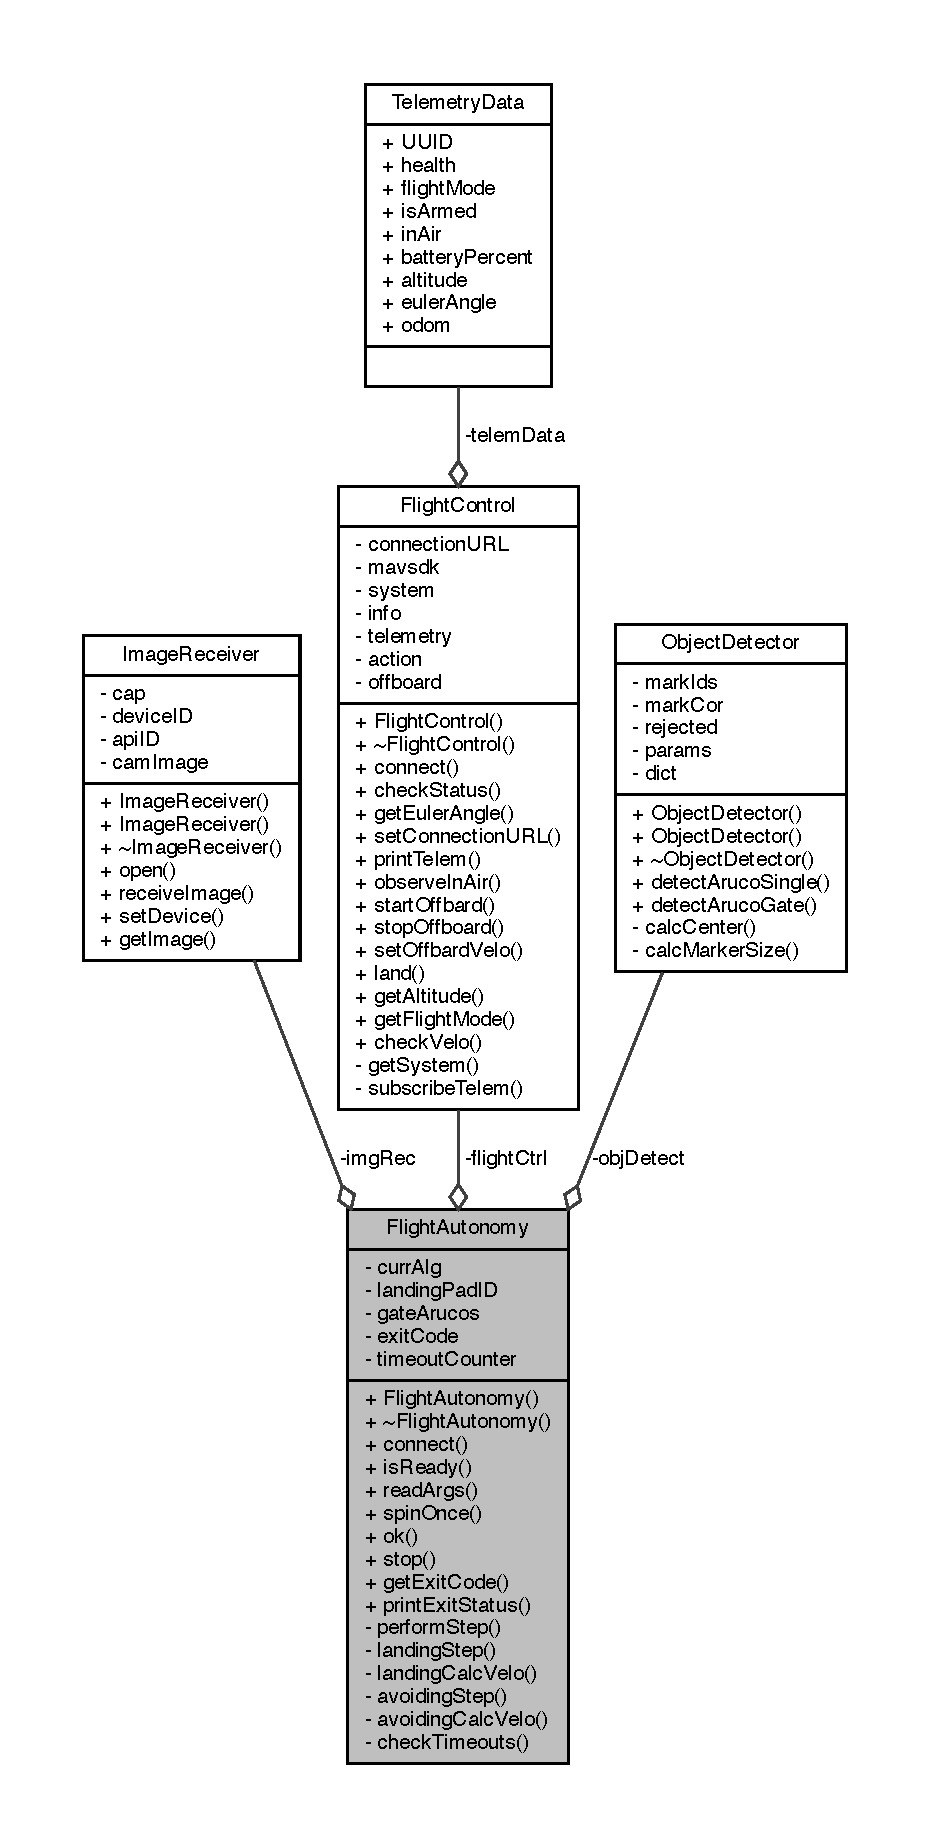
\includegraphics[height=550pt]{classFlightAutonomy__coll__graph}
\end{center}
\end{figure}
\doxysubsubsection*{Metody publiczne}
\begin{DoxyCompactItemize}
\item 
\mbox{\hyperlink{classFlightAutonomy_a8040acc62f429cb0d8d1d97b7343baf6}{Flight\+Autonomy}} ()
\begin{DoxyCompactList}\small\item\em Konstruuje obiekt \mbox{\hyperlink{classFlightAutonomy}{Flight\+Autonomy}} inicjalizując pola domyślnymi wartościami. \end{DoxyCompactList}\item 
\mbox{\hyperlink{classFlightAutonomy_a28cfb113ef95851ad015666c4a64cb11}{$\sim$\+Flight\+Autonomy}} ()
\begin{DoxyCompactList}\small\item\em Destuktor. W trybie debugowania niszczący okno Open\+CV. \end{DoxyCompactList}\item 
bool \mbox{\hyperlink{classFlightAutonomy_ad349e89e1057ff74edb31cf802ec0fa8}{connect}} ()
\begin{DoxyCompactList}\small\item\em Inicjalizuje połączenie z autopilotem poprzez protokół Mav\+Link oraz uruchamia tryb offboard. \end{DoxyCompactList}\item 
bool \mbox{\hyperlink{classFlightAutonomy_a0f3696b3824356b430a8e984bff183bb}{is\+Ready}} ()
\begin{DoxyCompactList}\small\item\em Sprawdza czy maszyna jest gotowa do wykonywania algorytmu. \end{DoxyCompactList}\item 
bool \mbox{\hyperlink{classFlightAutonomy_a3021f6ccd2017c1ddf9cf5610817fe00}{read\+Args}} (const int argc, char $\ast$$\ast$argv)
\begin{DoxyCompactList}\small\item\em Wczytuje przekazane do programu parametry. \end{DoxyCompactList}\item 
bool \mbox{\hyperlink{classFlightAutonomy_a619dfe9c6378206dd8bc2c7cd2a8736f}{spin\+Once}} ()
\begin{DoxyCompactList}\small\item\em Wykonuje pojedynczy krok algorytmu. Powinna być wywoływana jednokrotnie w trakcie każdego obrotu pętli głównej programu. \end{DoxyCompactList}\item 
bool \mbox{\hyperlink{classFlightAutonomy_a809a057eb8ad54e566783487c91c5aed}{ok}} ()
\begin{DoxyCompactList}\small\item\em Sprawdza czy wszystkie elementy działają prawidłowo i czy nie pojawił się warunek wyjścia. \end{DoxyCompactList}\item 
bool \mbox{\hyperlink{classFlightAutonomy_a46c04fee7163ea940587c977358df0a5}{stop}} ()
\begin{DoxyCompactList}\small\item\em Kończy działanie algorytmu i wyłącza tryb offboard. \end{DoxyCompactList}\item 
int \mbox{\hyperlink{classFlightAutonomy_a0730076c08f380927ab55ef2db930370}{get\+Exit\+Code}} ()
\begin{DoxyCompactList}\small\item\em Zwraca wartość kodu wyjścia. \end{DoxyCompactList}\item 
void \mbox{\hyperlink{classFlightAutonomy_aeb94cacda630ffcc60a89d17f46f9965}{print\+Exit\+Status}} ()
\begin{DoxyCompactList}\small\item\em Wyświetla status wyjścia według kodu w zmiennej exit\+Code. \end{DoxyCompactList}\end{DoxyCompactItemize}
\doxysubsubsection*{Metody prywatne}
\begin{DoxyCompactItemize}
\item 
int \mbox{\hyperlink{classFlightAutonomy_adebcdd60f50853bb8f8de0a13ba5792c}{perform\+Step}} (cv\+::\+Mat \&img)
\begin{DoxyCompactList}\small\item\em Wykonuje pojedyncza iterację dla wybranego algorytmu. \end{DoxyCompactList}\item 
bool \mbox{\hyperlink{classFlightAutonomy_a52d5d6ae4ad61e11abf7d851578747fc}{landing\+Step}} (cv\+::\+Mat \&img)
\begin{DoxyCompactList}\small\item\em Wykonuje jeden krok algorytmu lądowania. \end{DoxyCompactList}\item 
mavsdk\+::\+Offboard\+::\+Velocity\+Body\+Yawspeed \mbox{\hyperlink{classFlightAutonomy_ab440b55d8bce5238dea41278e1a4dd8b}{landing\+Calc\+Velo}} (cv\+::\+Mat \&img, cv\+::\+Point2f aruco\+Position)
\begin{DoxyCompactList}\small\item\em Oblicza prędkości danej iteracji algorytmu lądowania. \end{DoxyCompactList}\item 
bool \mbox{\hyperlink{classFlightAutonomy_a8d5d37d1c1fd723b4dffcc00d442cb2e}{avoiding\+Step}} (cv\+::\+Mat \&img)
\begin{DoxyCompactList}\small\item\em Wykonuje jeden krok algorytmu lądowania. \end{DoxyCompactList}\item 
mavsdk\+::\+Offboard\+::\+Velocity\+Body\+Yawspeed \mbox{\hyperlink{classFlightAutonomy_abd83d4b9055c8519149539af79eb932a}{avoiding\+Calc\+Velo}} (cv\+::\+Mat \&img, cv\+::\+Point2f gate\+Position, float angle)
\begin{DoxyCompactList}\small\item\em Oblicza prędkości danej iteracji algorytmu przelotu przez bramkę, potrzebne do przelotu przez bramkę. \end{DoxyCompactList}\item 
void \mbox{\hyperlink{classFlightAutonomy_af65554f658cc6baaee03386973516623}{check\+Timeouts}} ()
\begin{DoxyCompactList}\small\item\em Sprawdza czy nastąpiło przekroczenie zdefiniowanych czasów maksymalnych. \end{DoxyCompactList}\end{DoxyCompactItemize}
\doxysubsubsection*{Atrybuty prywatne}
\begin{DoxyCompactItemize}
\item 
\mbox{\hyperlink{classImageReceiver}{Image\+Receiver}} \mbox{\hyperlink{classFlightAutonomy_ac77d9e7161595e6add998d41c6af2865}{img\+Rec}}
\begin{DoxyCompactList}\small\item\em Odbiornik obrazu z kamery. \end{DoxyCompactList}\item 
\mbox{\hyperlink{classFlightControl}{Flight\+Control}} \mbox{\hyperlink{classFlightAutonomy_adb7277ac2f2610d32a742eac6e2547af}{flight\+Ctrl}}
\begin{DoxyCompactList}\small\item\em Kontrola lotu maszyny. \end{DoxyCompactList}\item 
\mbox{\hyperlink{classObjectDetector}{Object\+Detector}} \mbox{\hyperlink{classFlightAutonomy_a009d1c5234a6092c5265ebdcecdd48d7}{obj\+Detect}}
\begin{DoxyCompactList}\small\item\em Wykrywacz obiektów na obrazie z kamery. \end{DoxyCompactList}\item 
\mbox{\hyperlink{algorithms_8h_a269b54498ecf7693a990d2002e0e9ca0}{Algorithms}} \mbox{\hyperlink{classFlightAutonomy_a48e558c247c415586cb0b178a0eb362f}{curr\+Alg}}
\begin{DoxyCompactList}\small\item\em Obecnie wykonywany algorytm. \end{DoxyCompactList}\item 
int \mbox{\hyperlink{classFlightAutonomy_a8c699b95deba4b7a78758d6e8d3f7acc}{landing\+Pad\+ID}} = 68
\begin{DoxyCompactList}\small\item\em ID znacznika Aruco lądowiska. \end{DoxyCompactList}\item 
int \mbox{\hyperlink{classFlightAutonomy_a584c7377b13189eea602a4e607ca2a41}{gate\+Arucos}} \mbox{[}4\mbox{]} = \{10, 11, 12, 13\}
\begin{DoxyCompactList}\small\item\em ID znaczników umieszczonych na bramce zgodnie z ruchem wskazówek zegara. \end{DoxyCompactList}\item 
int \mbox{\hyperlink{classFlightAutonomy_a739dbb496b8c2fbd23a6d3e736a78586}{exit\+Code}}
\begin{DoxyCompactList}\small\item\em Kod wyjścia z systemu\+: 0 -\/ kontynuuj pracę, 1 -\/ wyjście normalne, 2 -\/ niepoprawna wysokość, 3 -\/ nie wykryto znaczników przez zadany czas. \end{DoxyCompactList}\item 
std\+::chrono\+::steady\+\_\+clock\+::time\+\_\+point \mbox{\hyperlink{classFlightAutonomy_a4f1a1408f0d491c6a2e9acecab30711e}{timeout\+Counter}}
\begin{DoxyCompactList}\small\item\em Odlicza czas do automatycznego wyjścia z programu w przypadku nie wykrywania znaczników. \end{DoxyCompactList}\end{DoxyCompactItemize}


\doxysubsubsection{Opis szczegółowy}
Klasa odpowiedzialna za kompleksową obsługę autonomii lotu bazującej na analizie wizyjnej. W klasie realizowany jest algorytm analizujący obraz odbierany z kamery i w przypadku wykrycia przeszkody wykonanie odpowiedniej reakcji w postaci zmiany trajektorii lotu maszyny. Wykorzystywany jest protokół Mav\+Link do dwukierunkowej komunikacji z autopilotem i przesyłania komend sterujących. 

\doxysubsubsection{Dokumentacja konstruktora i destruktora}
\mbox{\Hypertarget{classFlightAutonomy_a8040acc62f429cb0d8d1d97b7343baf6}\label{classFlightAutonomy_a8040acc62f429cb0d8d1d97b7343baf6}} 
\index{FlightAutonomy@{FlightAutonomy}!FlightAutonomy@{FlightAutonomy}}
\index{FlightAutonomy@{FlightAutonomy}!FlightAutonomy@{FlightAutonomy}}
\doxyparagraph{\texorpdfstring{FlightAutonomy()}{FlightAutonomy()}}
{\footnotesize\ttfamily Flight\+Autonomy\+::\+Flight\+Autonomy (\begin{DoxyParamCaption}{ }\end{DoxyParamCaption})}



Konstruuje obiekt \mbox{\hyperlink{classFlightAutonomy}{Flight\+Autonomy}} inicjalizując pola domyślnymi wartościami. 

\mbox{\Hypertarget{classFlightAutonomy_a28cfb113ef95851ad015666c4a64cb11}\label{classFlightAutonomy_a28cfb113ef95851ad015666c4a64cb11}} 
\index{FlightAutonomy@{FlightAutonomy}!````~FlightAutonomy@{$\sim$FlightAutonomy}}
\index{````~FlightAutonomy@{$\sim$FlightAutonomy}!FlightAutonomy@{FlightAutonomy}}
\doxyparagraph{\texorpdfstring{$\sim$FlightAutonomy()}{~FlightAutonomy()}}
{\footnotesize\ttfamily Flight\+Autonomy\+::$\sim$\+Flight\+Autonomy (\begin{DoxyParamCaption}{ }\end{DoxyParamCaption})}



Destuktor. W trybie debugowania niszczący okno Open\+CV. 



\doxysubsubsection{Dokumentacja funkcji składowych}
\mbox{\Hypertarget{classFlightAutonomy_abd83d4b9055c8519149539af79eb932a}\label{classFlightAutonomy_abd83d4b9055c8519149539af79eb932a}} 
\index{FlightAutonomy@{FlightAutonomy}!avoidingCalcVelo@{avoidingCalcVelo}}
\index{avoidingCalcVelo@{avoidingCalcVelo}!FlightAutonomy@{FlightAutonomy}}
\doxyparagraph{\texorpdfstring{avoidingCalcVelo()}{avoidingCalcVelo()}}
{\footnotesize\ttfamily mavsdk\+::\+Offboard\+::\+Velocity\+Body\+Yawspeed Flight\+Autonomy\+::avoiding\+Calc\+Velo (\begin{DoxyParamCaption}\item[{cv\+::\+Mat \&}]{img,  }\item[{cv\+::\+Point2f}]{gate\+Position,  }\item[{float}]{angle }\end{DoxyParamCaption})\hspace{0.3cm}{\ttfamily [private]}}



Oblicza prędkości danej iteracji algorytmu przelotu przez bramkę, potrzebne do przelotu przez bramkę. 


\begin{DoxyParams}{Parametry}
{\em img} & Przetwarzana ramka obrazu. \\
\hline
{\em gate\+Position} & Pozycja bramki na obrazie. \\
\hline
{\em angle} & Kąt pochylenia bramki. \\
\hline
\end{DoxyParams}
\begin{DoxyReturn}{Zwraca}
mavsdk\+::\+Offboard\+::\+Velocity\+Body\+Yawspeed 
\end{DoxyReturn}
\mbox{\Hypertarget{classFlightAutonomy_a8d5d37d1c1fd723b4dffcc00d442cb2e}\label{classFlightAutonomy_a8d5d37d1c1fd723b4dffcc00d442cb2e}} 
\index{FlightAutonomy@{FlightAutonomy}!avoidingStep@{avoidingStep}}
\index{avoidingStep@{avoidingStep}!FlightAutonomy@{FlightAutonomy}}
\doxyparagraph{\texorpdfstring{avoidingStep()}{avoidingStep()}}
{\footnotesize\ttfamily bool Flight\+Autonomy\+::avoiding\+Step (\begin{DoxyParamCaption}\item[{cv\+::\+Mat \&}]{img }\end{DoxyParamCaption})\hspace{0.3cm}{\ttfamily [private]}}



Wykonuje jeden krok algorytmu lądowania. 


\begin{DoxyParams}{Parametry}
{\em img} & Najnowsza ramka obrazu.\\
\hline
\end{DoxyParams}
\begin{DoxyReturn}{Zwraca}
true Poprawnie wykonano krok algorytmu. 

false Błąd podczas wykonywania kroku algorytmu. 
\end{DoxyReturn}
\mbox{\Hypertarget{classFlightAutonomy_af65554f658cc6baaee03386973516623}\label{classFlightAutonomy_af65554f658cc6baaee03386973516623}} 
\index{FlightAutonomy@{FlightAutonomy}!checkTimeouts@{checkTimeouts}}
\index{checkTimeouts@{checkTimeouts}!FlightAutonomy@{FlightAutonomy}}
\doxyparagraph{\texorpdfstring{checkTimeouts()}{checkTimeouts()}}
{\footnotesize\ttfamily void Flight\+Autonomy\+::check\+Timeouts (\begin{DoxyParamCaption}{ }\end{DoxyParamCaption})\hspace{0.3cm}{\ttfamily [private]}}



Sprawdza czy nastąpiło przekroczenie zdefiniowanych czasów maksymalnych. 

\mbox{\Hypertarget{classFlightAutonomy_ad349e89e1057ff74edb31cf802ec0fa8}\label{classFlightAutonomy_ad349e89e1057ff74edb31cf802ec0fa8}} 
\index{FlightAutonomy@{FlightAutonomy}!connect@{connect}}
\index{connect@{connect}!FlightAutonomy@{FlightAutonomy}}
\doxyparagraph{\texorpdfstring{connect()}{connect()}}
{\footnotesize\ttfamily bool Flight\+Autonomy\+::connect (\begin{DoxyParamCaption}{ }\end{DoxyParamCaption})}



Inicjalizuje połączenie z autopilotem poprzez protokół Mav\+Link oraz uruchamia tryb offboard. 

\begin{DoxyReturn}{Zwraca}
true Połączenie zostało nawiązane. 

false Wystąpił błąd podczas nawiązywania połączenia. 
\end{DoxyReturn}
\mbox{\Hypertarget{classFlightAutonomy_a0730076c08f380927ab55ef2db930370}\label{classFlightAutonomy_a0730076c08f380927ab55ef2db930370}} 
\index{FlightAutonomy@{FlightAutonomy}!getExitCode@{getExitCode}}
\index{getExitCode@{getExitCode}!FlightAutonomy@{FlightAutonomy}}
\doxyparagraph{\texorpdfstring{getExitCode()}{getExitCode()}}
{\footnotesize\ttfamily int Flight\+Autonomy\+::get\+Exit\+Code (\begin{DoxyParamCaption}{ }\end{DoxyParamCaption})}



Zwraca wartość kodu wyjścia. 

\begin{DoxyReturn}{Zwraca}
int Wartość kodu wyjścia. 
\end{DoxyReturn}
\mbox{\Hypertarget{classFlightAutonomy_a0f3696b3824356b430a8e984bff183bb}\label{classFlightAutonomy_a0f3696b3824356b430a8e984bff183bb}} 
\index{FlightAutonomy@{FlightAutonomy}!isReady@{isReady}}
\index{isReady@{isReady}!FlightAutonomy@{FlightAutonomy}}
\doxyparagraph{\texorpdfstring{isReady()}{isReady()}}
{\footnotesize\ttfamily bool Flight\+Autonomy\+::is\+Ready (\begin{DoxyParamCaption}{ }\end{DoxyParamCaption})}



Sprawdza czy maszyna jest gotowa do wykonywania algorytmu. 

\begin{DoxyReturn}{Zwraca}
true Maszyna jest gotowa. 

false Maszyna nie jest gotowa. 
\end{DoxyReturn}
\mbox{\Hypertarget{classFlightAutonomy_ab440b55d8bce5238dea41278e1a4dd8b}\label{classFlightAutonomy_ab440b55d8bce5238dea41278e1a4dd8b}} 
\index{FlightAutonomy@{FlightAutonomy}!landingCalcVelo@{landingCalcVelo}}
\index{landingCalcVelo@{landingCalcVelo}!FlightAutonomy@{FlightAutonomy}}
\doxyparagraph{\texorpdfstring{landingCalcVelo()}{landingCalcVelo()}}
{\footnotesize\ttfamily mavsdk\+::\+Offboard\+::\+Velocity\+Body\+Yawspeed Flight\+Autonomy\+::landing\+Calc\+Velo (\begin{DoxyParamCaption}\item[{cv\+::\+Mat \&}]{img,  }\item[{cv\+::\+Point2f}]{aruco\+Position }\end{DoxyParamCaption})\hspace{0.3cm}{\ttfamily [private]}}



Oblicza prędkości danej iteracji algorytmu lądowania. 


\begin{DoxyParams}{Parametry}
{\em img} & Przetwarzana ramka obrazu. \\
\hline
{\em aruco\+Position} & Pozycja znacznika lądowiska na obrazie. \\
\hline
\end{DoxyParams}
\begin{DoxyReturn}{Zwraca}
mavsdk\+::\+Offboard\+::\+Velocity\+Body\+Yawspeed 
\end{DoxyReturn}
\mbox{\Hypertarget{classFlightAutonomy_a52d5d6ae4ad61e11abf7d851578747fc}\label{classFlightAutonomy_a52d5d6ae4ad61e11abf7d851578747fc}} 
\index{FlightAutonomy@{FlightAutonomy}!landingStep@{landingStep}}
\index{landingStep@{landingStep}!FlightAutonomy@{FlightAutonomy}}
\doxyparagraph{\texorpdfstring{landingStep()}{landingStep()}}
{\footnotesize\ttfamily bool Flight\+Autonomy\+::landing\+Step (\begin{DoxyParamCaption}\item[{cv\+::\+Mat \&}]{img }\end{DoxyParamCaption})\hspace{0.3cm}{\ttfamily [private]}}



Wykonuje jeden krok algorytmu lądowania. 


\begin{DoxyParams}{Parametry}
{\em img} & Najnowsza ramka obrazu.\\
\hline
\end{DoxyParams}
\begin{DoxyReturn}{Zwraca}
true Poprawnie wykonano krok algorytmu. 

false Błąd podczas wykonywania kroku algorytmu. 
\end{DoxyReturn}
\mbox{\Hypertarget{classFlightAutonomy_a809a057eb8ad54e566783487c91c5aed}\label{classFlightAutonomy_a809a057eb8ad54e566783487c91c5aed}} 
\index{FlightAutonomy@{FlightAutonomy}!ok@{ok}}
\index{ok@{ok}!FlightAutonomy@{FlightAutonomy}}
\doxyparagraph{\texorpdfstring{ok()}{ok()}}
{\footnotesize\ttfamily bool Flight\+Autonomy\+::ok (\begin{DoxyParamCaption}{ }\end{DoxyParamCaption})}



Sprawdza czy wszystkie elementy działają prawidłowo i czy nie pojawił się warunek wyjścia. 

\begin{DoxyReturn}{Zwraca}
true Wszystkie komponenty działają prawidłowo i nie pojawił się warunek wyjścia. 

false Pojawił się błąd działania lub warunek wyjścia. 
\end{DoxyReturn}
\mbox{\Hypertarget{classFlightAutonomy_adebcdd60f50853bb8f8de0a13ba5792c}\label{classFlightAutonomy_adebcdd60f50853bb8f8de0a13ba5792c}} 
\index{FlightAutonomy@{FlightAutonomy}!performStep@{performStep}}
\index{performStep@{performStep}!FlightAutonomy@{FlightAutonomy}}
\doxyparagraph{\texorpdfstring{performStep()}{performStep()}}
{\footnotesize\ttfamily int Flight\+Autonomy\+::perform\+Step (\begin{DoxyParamCaption}\item[{cv\+::\+Mat \&}]{img }\end{DoxyParamCaption})\hspace{0.3cm}{\ttfamily [private]}}



Wykonuje pojedyncza iterację dla wybranego algorytmu. 


\begin{DoxyParams}{Parametry}
{\em img} & Najnowsza odebrana ramka obrazu.\\
\hline
\end{DoxyParams}
\begin{DoxyReturn}{Zwraca}
int Kod zwrócony przez algorytm. 
\end{DoxyReturn}
\mbox{\Hypertarget{classFlightAutonomy_aeb94cacda630ffcc60a89d17f46f9965}\label{classFlightAutonomy_aeb94cacda630ffcc60a89d17f46f9965}} 
\index{FlightAutonomy@{FlightAutonomy}!printExitStatus@{printExitStatus}}
\index{printExitStatus@{printExitStatus}!FlightAutonomy@{FlightAutonomy}}
\doxyparagraph{\texorpdfstring{printExitStatus()}{printExitStatus()}}
{\footnotesize\ttfamily void Flight\+Autonomy\+::print\+Exit\+Status (\begin{DoxyParamCaption}{ }\end{DoxyParamCaption})}



Wyświetla status wyjścia według kodu w zmiennej exit\+Code. 

\mbox{\Hypertarget{classFlightAutonomy_a3021f6ccd2017c1ddf9cf5610817fe00}\label{classFlightAutonomy_a3021f6ccd2017c1ddf9cf5610817fe00}} 
\index{FlightAutonomy@{FlightAutonomy}!readArgs@{readArgs}}
\index{readArgs@{readArgs}!FlightAutonomy@{FlightAutonomy}}
\doxyparagraph{\texorpdfstring{readArgs()}{readArgs()}}
{\footnotesize\ttfamily bool Flight\+Autonomy\+::read\+Args (\begin{DoxyParamCaption}\item[{const int}]{argc,  }\item[{char $\ast$$\ast$}]{argv }\end{DoxyParamCaption})}



Wczytuje przekazane do programu parametry. 


\begin{DoxyParams}{Parametry}
{\em argc} & Liczba parametrów \\
\hline
{\em argv} & Wskaźnik na tablicę parametrów\\
\hline
\end{DoxyParams}
\begin{DoxyReturn}{Zwraca}
true Poprawnie wczytano parametry. 

false Nie można wczytać parametrów. 
\end{DoxyReturn}
\mbox{\Hypertarget{classFlightAutonomy_a619dfe9c6378206dd8bc2c7cd2a8736f}\label{classFlightAutonomy_a619dfe9c6378206dd8bc2c7cd2a8736f}} 
\index{FlightAutonomy@{FlightAutonomy}!spinOnce@{spinOnce}}
\index{spinOnce@{spinOnce}!FlightAutonomy@{FlightAutonomy}}
\doxyparagraph{\texorpdfstring{spinOnce()}{spinOnce()}}
{\footnotesize\ttfamily bool Flight\+Autonomy\+::spin\+Once (\begin{DoxyParamCaption}{ }\end{DoxyParamCaption})}



Wykonuje pojedynczy krok algorytmu. Powinna być wywoływana jednokrotnie w trakcie każdego obrotu pętli głównej programu. 

\mbox{\Hypertarget{classFlightAutonomy_a46c04fee7163ea940587c977358df0a5}\label{classFlightAutonomy_a46c04fee7163ea940587c977358df0a5}} 
\index{FlightAutonomy@{FlightAutonomy}!stop@{stop}}
\index{stop@{stop}!FlightAutonomy@{FlightAutonomy}}
\doxyparagraph{\texorpdfstring{stop()}{stop()}}
{\footnotesize\ttfamily bool Flight\+Autonomy\+::stop (\begin{DoxyParamCaption}{ }\end{DoxyParamCaption})}



Kończy działanie algorytmu i wyłącza tryb offboard. 

\begin{DoxyReturn}{Zwraca}
true Pomyślnie zakończono działanie. 

false Pojawił się błąd podczas próby zakończenia działania. 
\end{DoxyReturn}


\doxysubsubsection{Dokumentacja atrybutów składowych}
\mbox{\Hypertarget{classFlightAutonomy_a48e558c247c415586cb0b178a0eb362f}\label{classFlightAutonomy_a48e558c247c415586cb0b178a0eb362f}} 
\index{FlightAutonomy@{FlightAutonomy}!currAlg@{currAlg}}
\index{currAlg@{currAlg}!FlightAutonomy@{FlightAutonomy}}
\doxyparagraph{\texorpdfstring{currAlg}{currAlg}}
{\footnotesize\ttfamily \mbox{\hyperlink{algorithms_8h_a269b54498ecf7693a990d2002e0e9ca0}{Algorithms}} Flight\+Autonomy\+::curr\+Alg\hspace{0.3cm}{\ttfamily [private]}}



Obecnie wykonywany algorytm. 

\mbox{\Hypertarget{classFlightAutonomy_a739dbb496b8c2fbd23a6d3e736a78586}\label{classFlightAutonomy_a739dbb496b8c2fbd23a6d3e736a78586}} 
\index{FlightAutonomy@{FlightAutonomy}!exitCode@{exitCode}}
\index{exitCode@{exitCode}!FlightAutonomy@{FlightAutonomy}}
\doxyparagraph{\texorpdfstring{exitCode}{exitCode}}
{\footnotesize\ttfamily int Flight\+Autonomy\+::exit\+Code\hspace{0.3cm}{\ttfamily [private]}}



Kod wyjścia z systemu\+: 0 -\/ kontynuuj pracę, 1 -\/ wyjście normalne, 2 -\/ niepoprawna wysokość, 3 -\/ nie wykryto znaczników przez zadany czas. 

\mbox{\Hypertarget{classFlightAutonomy_adb7277ac2f2610d32a742eac6e2547af}\label{classFlightAutonomy_adb7277ac2f2610d32a742eac6e2547af}} 
\index{FlightAutonomy@{FlightAutonomy}!flightCtrl@{flightCtrl}}
\index{flightCtrl@{flightCtrl}!FlightAutonomy@{FlightAutonomy}}
\doxyparagraph{\texorpdfstring{flightCtrl}{flightCtrl}}
{\footnotesize\ttfamily \mbox{\hyperlink{classFlightControl}{Flight\+Control}} Flight\+Autonomy\+::flight\+Ctrl\hspace{0.3cm}{\ttfamily [private]}}



Kontrola lotu maszyny. 

\mbox{\Hypertarget{classFlightAutonomy_a584c7377b13189eea602a4e607ca2a41}\label{classFlightAutonomy_a584c7377b13189eea602a4e607ca2a41}} 
\index{FlightAutonomy@{FlightAutonomy}!gateArucos@{gateArucos}}
\index{gateArucos@{gateArucos}!FlightAutonomy@{FlightAutonomy}}
\doxyparagraph{\texorpdfstring{gateArucos}{gateArucos}}
{\footnotesize\ttfamily int Flight\+Autonomy\+::gate\+Arucos\mbox{[}4\mbox{]} = \{10, 11, 12, 13\}\hspace{0.3cm}{\ttfamily [private]}}



ID znaczników umieszczonych na bramce zgodnie z ruchem wskazówek zegara. 

\mbox{\Hypertarget{classFlightAutonomy_ac77d9e7161595e6add998d41c6af2865}\label{classFlightAutonomy_ac77d9e7161595e6add998d41c6af2865}} 
\index{FlightAutonomy@{FlightAutonomy}!imgRec@{imgRec}}
\index{imgRec@{imgRec}!FlightAutonomy@{FlightAutonomy}}
\doxyparagraph{\texorpdfstring{imgRec}{imgRec}}
{\footnotesize\ttfamily \mbox{\hyperlink{classImageReceiver}{Image\+Receiver}} Flight\+Autonomy\+::img\+Rec\hspace{0.3cm}{\ttfamily [private]}}



Odbiornik obrazu z kamery. 

\mbox{\Hypertarget{classFlightAutonomy_a8c699b95deba4b7a78758d6e8d3f7acc}\label{classFlightAutonomy_a8c699b95deba4b7a78758d6e8d3f7acc}} 
\index{FlightAutonomy@{FlightAutonomy}!landingPadID@{landingPadID}}
\index{landingPadID@{landingPadID}!FlightAutonomy@{FlightAutonomy}}
\doxyparagraph{\texorpdfstring{landingPadID}{landingPadID}}
{\footnotesize\ttfamily int Flight\+Autonomy\+::landing\+Pad\+ID = 68\hspace{0.3cm}{\ttfamily [private]}}



ID znacznika Aruco lądowiska. 

\mbox{\Hypertarget{classFlightAutonomy_a009d1c5234a6092c5265ebdcecdd48d7}\label{classFlightAutonomy_a009d1c5234a6092c5265ebdcecdd48d7}} 
\index{FlightAutonomy@{FlightAutonomy}!objDetect@{objDetect}}
\index{objDetect@{objDetect}!FlightAutonomy@{FlightAutonomy}}
\doxyparagraph{\texorpdfstring{objDetect}{objDetect}}
{\footnotesize\ttfamily \mbox{\hyperlink{classObjectDetector}{Object\+Detector}} Flight\+Autonomy\+::obj\+Detect\hspace{0.3cm}{\ttfamily [private]}}



Wykrywacz obiektów na obrazie z kamery. 

\mbox{\Hypertarget{classFlightAutonomy_a4f1a1408f0d491c6a2e9acecab30711e}\label{classFlightAutonomy_a4f1a1408f0d491c6a2e9acecab30711e}} 
\index{FlightAutonomy@{FlightAutonomy}!timeoutCounter@{timeoutCounter}}
\index{timeoutCounter@{timeoutCounter}!FlightAutonomy@{FlightAutonomy}}
\doxyparagraph{\texorpdfstring{timeoutCounter}{timeoutCounter}}
{\footnotesize\ttfamily std\+::chrono\+::steady\+\_\+clock\+::time\+\_\+point Flight\+Autonomy\+::timeout\+Counter\hspace{0.3cm}{\ttfamily [private]}}



Odlicza czas do automatycznego wyjścia z programu w przypadku nie wykrywania znaczników. 



Dokumentacja dla tej klasy została wygenerowana z plików\+:\begin{DoxyCompactItemize}
\item 
include/\+Flight\+Autonomy/\mbox{\hyperlink{FlightAutonomy_8h}{Flight\+Autonomy.\+h}}\item 
src/\mbox{\hyperlink{FlightAutonomy_8cpp}{Flight\+Autonomy.\+cpp}}\end{DoxyCompactItemize}

\hypertarget{classImageReceiver}{}\section{Image\+Receiver Class Reference}
\label{classImageReceiver}\index{Image\+Receiver@{Image\+Receiver}}


Image receiving class that supports diferrent types of imput video streams.  




{\ttfamily \#include $<$Image\+Receiver.\+h$>$}

\subsection*{Public Member Functions}
\begin{DoxyCompactItemize}
\item 
\mbox{\Hypertarget{classImageReceiver_ae1356643b5d08041070aee58e2294a59}\label{classImageReceiver_ae1356643b5d08041070aee58e2294a59}} 
{\bfseries Image\+Receiver} (ros\+::\+Node\+Handle \&\+\_\+nh, std\+::string topic)
\end{DoxyCompactItemize}


\subsection{Detailed Description}
Image receiving class that supports diferrent types of imput video streams. 

The documentation for this class was generated from the following files\+:\begin{DoxyCompactItemize}
\item 
include/Image\+Receiver.\+h\item 
src/Image\+Receiver.\+cpp\end{DoxyCompactItemize}

%--- End generated contents ---

% Index
\backmatter
\newpage
\phantomsection
\clearemptydoublepage
\addcontentsline{toc}{chapter}{Index}
\printindex

\end{document}
